\documentclass[a4paper,french,12pt]{article}
\usepackage{babel,amssymb,amsmath}
\usepackage[utf8]{inputenc}
\usepackage{array,colortbl}
\usepackage[T1]{fontenc}
\usepackage{multicol}
%\usepackage{multirow}
%\usepackage[8pt]{pstricks}
\usepackage{textcomp}
\usepackage{fancyhdr}
\usepackage{geometry}
\usepackage{eurosym}
% \usepackage{titling}
%\usepackage{makeidx}
% \usepackage[maxfloats=50]{morefloats}
% \usepackage{hyperref}
\usepackage{ulem}
 
\usepackage{epigraph}
\geometry{rmargin=2.5cm, lmargin=2.5cm, hmargin=2cm, bmargin=2cm}
\pagestyle{plain}
\usepackage[pdftex]{thumbpdf}
%\definecolor{vert}{rgb}{0.25,0.65,0.04}
\usepackage[pdftex,
    bookmarks         = true,
    bookmarksnumbered = true,
    pdfpagemode       = None,
    pdfstartview      = FitH,
    pdfpagelayout     = SinglePage,
    colorlinks        = true,
    linkcolor	      = black,
    pdfborder         = {0 0 0}
    ]{hyperref}
\usepackage{graphicx}
\usepackage[ruled]{algorithm2e}

\newcommand{\HRule}{\rule{\linewidth}{0.5mm}}
% \hypersetup{
% 	pdfauthor = {Philippe \textsc{GAULTIER}},
% 	pdftitle = {Rapport de stage du 17/06/2013 au 23/08/2013},
% 	pdfsubject = {},
% 	pdfkeywords = {},
% 	pdfcreator = {},
% }
% \newcommand{\filename}[1]{\textbf{\#1}}
% \newcommand{\fonction}[1]{\textbf{\itshape{\#1}}} 
% \newcommand{\tabl}[1]{\textbf{\itshape{\#1}}[ ]} 
\begin{document}
\begin{titlepage}
\begin{center}

%Logo

\includegraphics[width=0.4\textwidth]{./logo_ENSIIE.png}~\\[1cm]
\textsc{\huge Ensiie Strasbourg}\\[1.5cm]

%Title
\HRule \\[0.4cm]
{
	\huge \bfseries Rapport de stage
\\[0.4cm] }
\HRule \\[1.5cm]

% Author and supervisor
\begin{minipage}{0.4\textwidth}
\begin{flushleft} \huge
\emph{Auteur:}\\
Philippe \textsc{Gaultier},\\[0.5cm]
\Large élève ingénieur à l'Ensiie Strasbourg
\end{flushleft}
\end{minipage}
\begin{minipage}{0.4\textwidth}
\begin{flushright} \huge
\emph{Maître de stage:} \\
André \textsc{Schaaf},\\[0.5cm]
\Large enseignant-chercheur à l'Université de Strasbourg
\end{flushright}
\end{minipage}

\vfill

% Bottom of the page
{\large Strasbourg, le \today}



%\maketitle
% \theauthor
% \thetitle
% \thedate
% \makeindex
\end{center}
\end{titlepage}

\newpage
{
  \centering
  {
    \vspace{3cm}
    \epigraph{Always code as if the guy who ends up maintaining your code will be a violent psychopath who knows where you live}{Martin Golding}
    \vspace{3cm}
    \epigraph{The road is long and in the end the journey is the destination}{Unknown}
  }
}
\newpage
\textit{\normalsize Dans toute la suite du rapport, l'<<Observatoire>> désigne l'<<Observatoire astronomique de Strasbourg>>
et l'<<Unistra>> ou l'<<UDS>> désignent l'<<Université de Strasbourg>>.}
\setlength{\columnseprule}{0.5pt}
\tableofcontents

\newpage

\section{Introduction}

	L'Observatoire est un établissement de recherche et d'enseignement centré sur l'astronomie, mais c'est aussi un 
	centre de données astronomiques et un centre d'observation réputés mondialement. Il représente la continuité entre
	l'ancien et le nouveau car il dispose d'un riche patrimoine mais est aussi à la pointe de la recherche.  \\
	De plus l'Observatoire est le parfait exemple de l'informatique au service d'autres spécialités scientifiques,
	à la fois dans le domaine de l'expertise, mais aussi sous un aspect éducatif.\\
	Pour toutes ces raisons, j'ai choisi d'effectuer mon stage de deuxième année au sein de l'Observatoire,
	au contact de technologies émergentes à savoir l'Oculus Rift et le rendu graphique 3D moderne.

\section{Présentation de l'observatoire}

	\subsection{Histoire}
		L'Observatoire a été fondé en 1881 sur l'initiative de l'empereur Guillaume II, l'Alsace étant allemande
		à cette époque.\\
		Il est constitué de trois bâtiments : une Grande Coupole, un bâtiment des salles méridiennes avec deux coupoles,
		et un bâtiment à usage de bureau et de résidence.\\
		La Grande Coupole en fer, de 9,2 mètres de diamètre et pesant 34 tonnes2, contient le Grand Réfracteur,
		une lunette de 48,7 cm d'ouverture et 7 m de focale, construite en 1877, la plus grande d'Europe
		au moment de son installation et aujourd'hui (2008) la troisième de France en taille.\\
		Il dispose également d’un riche patrimoine d’instruments et d’ouvrage anciens.
		
	\subsection{Centre de données astronomiques de Strasbourg (CDS)}
	
		Le CDS est à la fois une équipe de recherche et un Service d’Observation.
		Les services de bases de données (SIMBAD, Vizier) et de visualisation (ALADIN) développés par le CDS
		sont utilisés par l’ensemble de la communauté astronomique mondiale. \\
		Celui-ci est l'un des acteurs majeurs du développement de l'Observatoire Virtuel International en astronomie.
		Fin 2008, le CDS a été labellisé TGIR (Très Grande Infrastructure de Recherche) par le Ministère de l'Enseignement Supérieur et de la Recherche, 
		reconfirmé comme Infrastructure de Recherche en 2012, ce qui le range au même niveau que des infrastructures internationales
		comme l’European Southern Observatory ou RENATER à l’échelon national.

	\subsection{Equipe de recherche Galaxies}
	
		L’équipe <<Galaxies>> étudie la formation et l’évolution des galaxies et de notre Galaxie 
		au travers de leurs populations stellaires et de la dynamique des étoiles et de la matière noire. \\
		Elle est impliquée dans la préparation de la mission satellitaire astrométrique Gaia de l’Agence Spatiale Européenne 
		dont le lancement est prévu en 2012 et dans le grand relevé cinématique RAVE. 
	
	\subsection{Equipe de recherche Hautes Énergies} 
	
		L’équipe <<Hautes Énergies>> s’intéresse aux sources galactiques et extragalactiques émettrices en rayons X,
		objets compacts (étoiles à neutron, naines blanches, etc.) et noyaux actifs de galaxies.\\
		Elle est impliquée dans le SSC-XMM, un consortium international de laboratoires sélectionné par l’ESA
		et labellisé par l’INSU comme Service d’Observation, qui est en charge de fournir des catalogues complets
		de sources X observées par le satellite XMM-Newton à la communauté internationale. 

\section{Mon stage}

	\subsection{Objectif}	
	
		L’objectif de ce stage a été centré autour de l'Oculus Rift et a été double:
		\begin{itemize}
		 \item Intégration de l'Oculus Rift à une simulation 3D du système solaire existante,
		 \item Développement d'un programme de visualisation 3D  d'étoiles avec intégration de l'Oculus Rift
		\end{itemize}
		
		J'ai donc travaillé sur deux projets distincts mais néanmoins complémentaires.
		
	    \subsubsection{Skybot 3D}
		Skybot 3D est un logiciel développé en C par l'institut de mécanique céleste et de calcul des éphémérides (IMCCE),
		conjointement avec l'Observatoire de Paris et le CNRS. Son propos est de faire un rendu graphique réaliste
		en 3D à partir des données célestes de ces instituts. En pratique, c'est une simulation 3D du système solaire
		où les échelles sont respectées.
		
		Mon travail a donc consisté en l'intégration du rendu Oculus dans cette application, tout en gardant
		le rendu existant.
		
	      
	    \subsubsection{Simulation}
		
	\subsection{L'Oculus Rift}
		
		\subsubsection{Aperçu}
		  L'Oculus Rift est un masque de réalité virtuelle, développé par \emph{Oculus VR}, une entreprise 
		  basée en Californie et rachetée par \emph{Facebook} en mars 2014 pour  2 milliards \$.
		  L'Oculus Rift a été initialement financé via une plateforme de financement collaboratif, \emph{Kickstarter},
		  et a levé 91 millions \$ à cette occasion. \\
		  Il permet une immersion  réaliste dans une scène en trois dimensions, en donnant l'impression d'y être physiquement
		  présent, et crée ainsi une nouvelle expérience
		  utilisateur. \\
		  De plus, son prix est relativement peu élevé (350 \$, environ 300 \euro), ce qui le rend accessible au grand public. \\
		  Pour toutes ces raisons, l'Oculus Rift est adapté à un usage éducatif et professionel, dans des domaines aussi variés
		  que la simulation scientifique, le divertissement, l'éducation, \ldots.
		  
		  La version grand public est prévue pour fin 2014 ou début 2015. J'ai pour ma part travaillé avec la première
		  version du masque, le \emph{DK1}, tandis que la deuxième version, le \emph{DK2} a été distribuée à partir d'août 2014.
		  
		  \begin{figure}[h!]
		    \centering
		      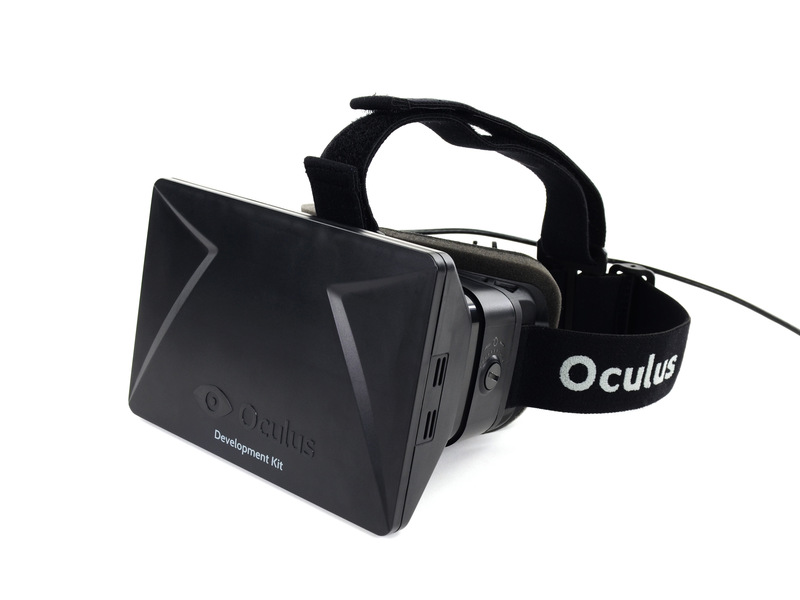
\includegraphics[width=0.3\textwidth]{dk1.jpg}
		    \caption{L'Oculus Rift (DK1)}
		  \end{figure}
		  
		  \subsubsection{Fonctionnement}
		  
			\paragraph{Matériel} ~\\
		    
				L'Oculus Rift est composé de:\\
			      
				\begin{itemize}
				\item Un écran 60 Hz d'une résolution de $1280*800$
				\item Deux lentilles (une pour chaque oeil),
				\item Un gyroscope à 3 axes pour mesurer l'accélération angulaire,
				\item Un magnétomètre à 3 axes pour mesurer les champs magnétiques,
				\item Un accéloromètre à 3 axes pour mesurer l'accélération, y compris gravitationnelle
				\item Un port USB
				\item Un port HDMI
				\end{itemize} ~
			       
				Il est à noter que la résolution de l'écran est à diviser par deux, chaque oeil voyant seulement
				une moitié de l'écran, la résolution effective est donc de $640*800$.
		    
			\paragraph{Logiciel} ~\\
			  
			    L'utilisation de l'Oculus Rift s'effectue au moyen de son SDK, qui permet:\\
			    
			    \begin{itemize}
			     \item D'accéder aux différents capteurs,
			     \item D'accéder aux propriétés du masque (distance inter-pupillaire, hauteur des yeux, \ldots),
			     \item D'appliquer les <<filtres>> au rendu graphique afin d'avoir un rendu réaliste
			    \end{itemize} ~
			    
			    Le SDK est écrit en C++ et possède une API en C.
			    Pour mon stage, j'ai utilisé la version 2.5 puis la version 0.3.2.
			
			\paragraph{Théorie} ~\\
			
			    L'Oculus Rift exige que la scène soit rendue graphiquement en <<split-screen stereo>>, 
			    c'est-à-dire avec l'écran divisé en deux verticalement, la partie gauche réservée à l'oeil gauche
			    et la partie droite à l'oeil droit.
			    
			    La distance inter-pupillaire est la distance entre les deux yeux. Elle varie d'un individu
			    à l'autre mais elle est en moyenne de 65 mm. Cette distance est importante dans le procédé 
			    de rendu car ce dernier consiste à rendre graphiquement la scène deux fois, une fois pour
			    chaque oeil, en translatant la caméra de la distance inter-pupillaire entre les deux rendus.
			    C'est ce qui contribue à créer l'effet stéréoscopique, ce qui crée l'impression d'immersion.
			
			    Un autre aspect à prendre en compte est la présence des lentilles. Ces dernières agrandissent
			    l'image pour fournir un champ de vision très large, pour améliorer l'immersion.
			    Cependant ce procédé déforme l'image de façon significative, ce qui créerait une distortion
			    en coussinets si les <<filtres>>, dont nous parleront plus tard,
			    n'étaient pas appliqués au niveau logiciel au rendu graphique de l'application.\\
			    
			     \begin{figure}[h!]
			      \centering
				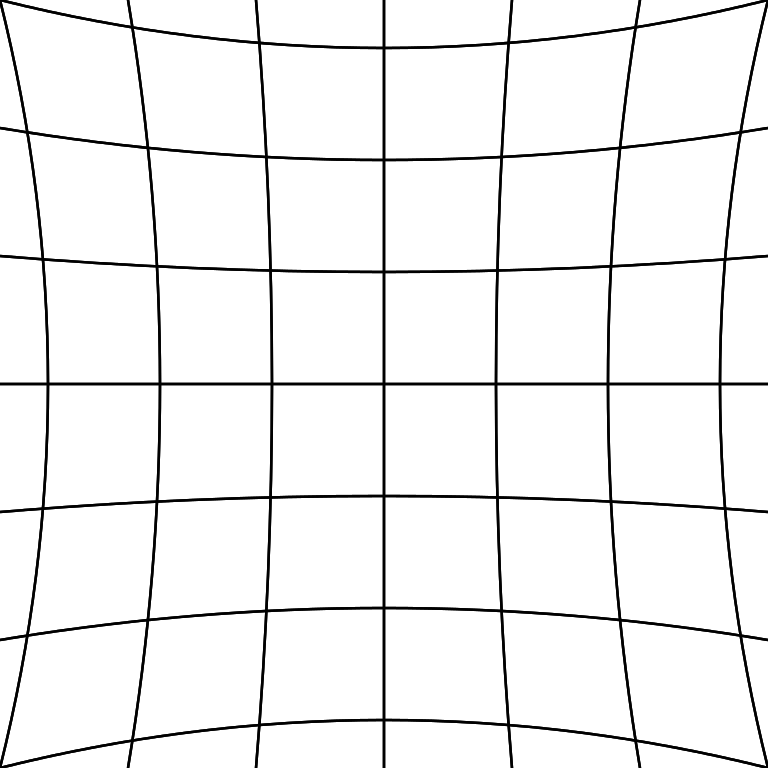
\includegraphics[width=3cm]{pincushion_distortion.png}
			      \caption{Distortion en coussinets (<<pincushion distortion>>)}\par\medskip
			    

			    Pour contrebalancer cette distortion, le programme doit, comme énoncé plus haut, appliquer
			    un effet post-rendu. Il s'agit d'une distortion égale et opposée, appelée distortion en 
			    barillets.\par\bigskip
			    
			     {
			      \centering
				
\includegraphics[width=3cm]{barrel_distortion.png}
			      \caption{Distortion en barillets (<<barrel distortion>>)}
			     }\par\medskip
			    
			    De plus, le programme doit corriger les aberrations chromatiques, qui consistent en un effet
			    d'arc en ciel aux contours des objets. Cet effet est causé par les lentilles.\par\bigskip
			    
			   {
			      \centering
				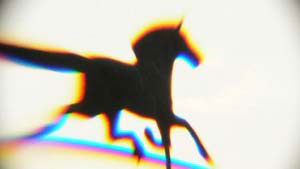
\includegraphics[width=4cm]{chromatic_aberration.jpg}
			      \caption{Aberration chromatique (<<chromatic abberration>>)}
			   }
			    \end{figure}  ~ \\
			    
			    
			\paragraph{Pratique} ~\\
			
			    Pour le développeur, ces éléments théoriques sont gérés de manière interne par le SDK Oculus.
			    
			    Pour une application qui fait un rendu graphique, la programme est typiquement de
			    la forme:\\
			    
			    \begin{algorithm}[H]
			      initialize the graphic resources\;
			      fill the scene with graphic objects\;
			      \While{the application is running}{
				process the user input\;
				update the objects in the scene\;
				render the objects in the scene\;
			      }
			      release the graphic resources\;
			      \caption{Application de rendu graphique}
			    \end{algorithm} ~\\
			    
			   
			    
			    
			    
			    Un programme qui fait un rendu Oculus exclusivement aura pour sa part la forme suivante:\\
			    
			    \begin{algorithm}[H]
			      initialize the graphic resources\;
			      initialize the Oculus SDK\;
			      fill the scene with graphic objects\;
			      \While{the application is running}{
				process the Oculus input\;
				update the objects in the scene\;
				\For{each eye}{
				  translate the camera by the inter-pupillary distance\;
				  apply the Oculus distortion effects\;
				  render the objects in the scene\;
				  }
			      }
			      release the Oculus SDK\;
			      release the graphic resources\;
			      \caption{Application de rendu graphique}
			    \end{algorithm} ~\\
			    Plus précisément, l'opération <<apply the Oculus distortion effects>> se fait de façon graphique
			    au moyen de shaders, qui sont des programmes qui appliquent des transformations à chaque pixel de l'image.
			    
			    
			    Nous avons alors le rendu suivant, pour une scène simple composée d'un cube texturé, d'un plan
			    et d'une skybox rudimentaire, avec le même point de vue:
			    
			    \clearpage
			    
			    \begin{figure}
			      \centering
				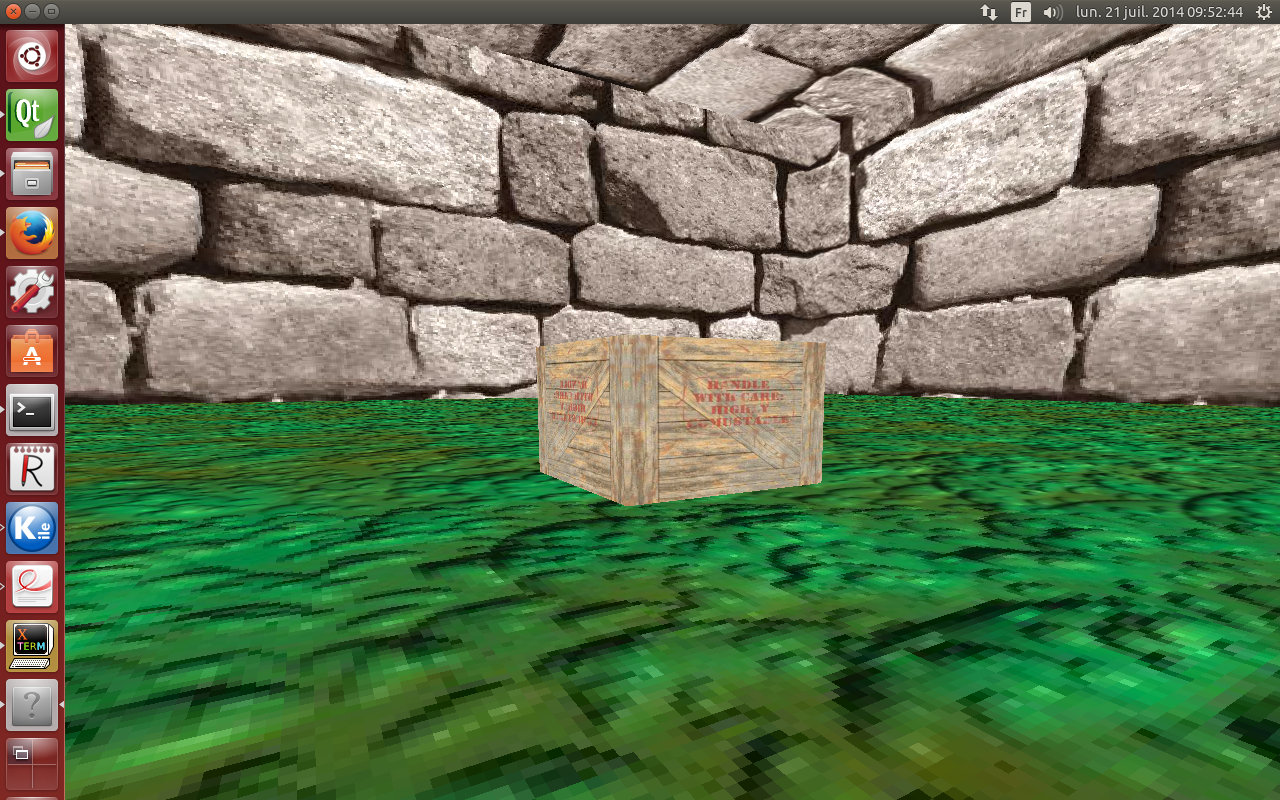
\includegraphics[width=1.0\textwidth]{scene_normal4.png}
			      \caption{Scène OpenGL simple avec le rendu normal}

				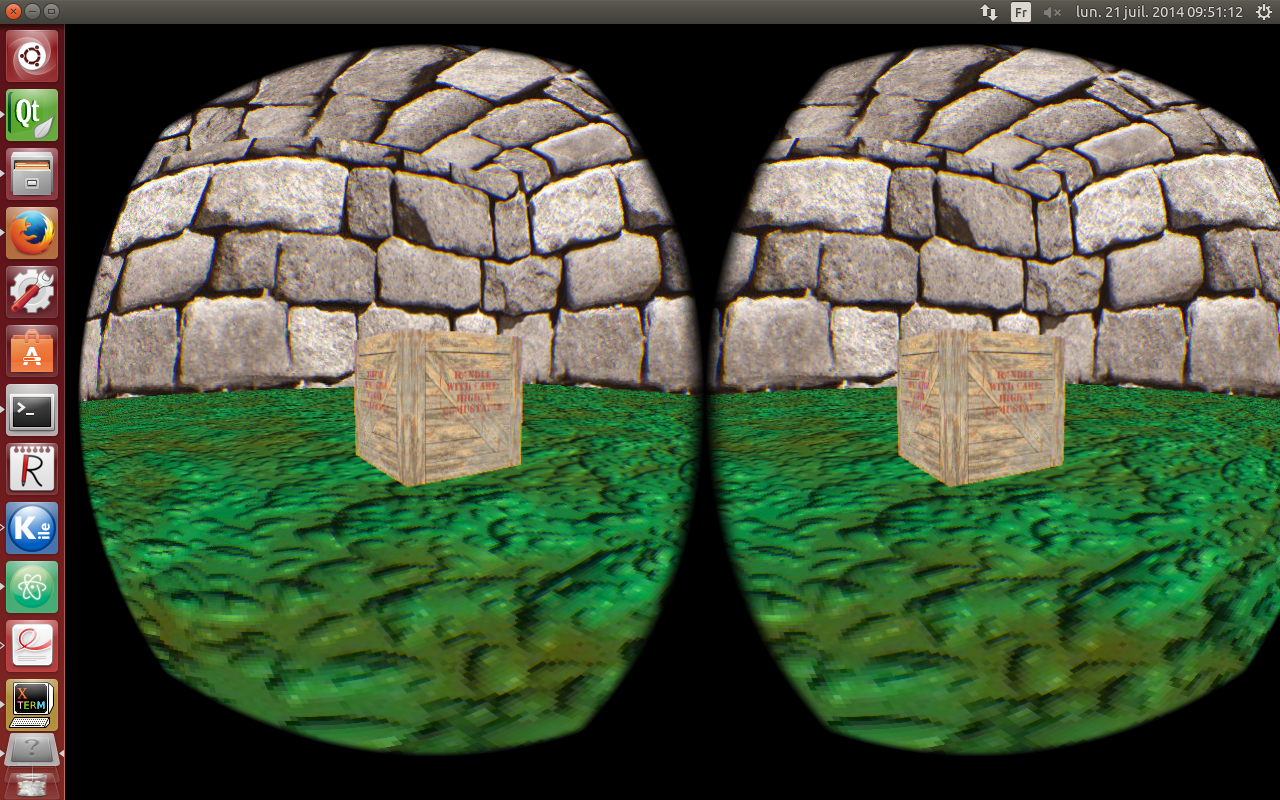
\includegraphics[width=1.0\textwidth]{scene_oculus4.png}
			      \caption{Scène OpenGL simple avec le rendu Oculus}
			    \end{figure}
			    \clearpage
			    
			    
			    
			    
			    Les applications que j'ai développées au sein de mon stage peuvent fournir le rendu normal 
			    et le rendu Oculus, selon l'option spécifiée.

		
	\subsection{Contraintes}
	
	  \subsubsection{Portabilité}
	  \subsubsection{Taille des données}
	  \subsubsection{Existant}


	\subsection{Outils utilisés}
	
		\subsubsection{Programmes utilisés}
		

		
		\subsubsection{Langages utilisés}
			
		

	
		\subsubsection{Bibliothèques utilisés}
		
		
	\subsection{Déroulement du stage}
	
		%Déroulement
	
	\subsection{Bonnes pratiques de développement}
			%Bonnes pratiques
	
	\subsection{Architecture}
	
  %Architecture de l'application

			
\section{Remerciements}

	Plusieurs personnes m’ont apporté une aide significative sur ce projet et je tiens à les remercier chaleureusement ici. 

	%Remerciements

  
  
\section{Conclusion}


		%Conclusion

% \appendix
\section{Annexes}
	
		\subsection{Captures d'écran}
		\newpage
		%Captures d'écran
	
	
	\subsection{Bibliographie}
	
		%Bibliographie

		
	\subsection{Glossaire}
		%Glossaire
		
\end{document}

